\documentclass[tikz,border=5pt]{standalone}
\usepackage{pgfplots}
\pgfplotsset{compat=1.18}
\definecolor{corba}{HTML}{365FB3}
\definecolor{punt}{HTML}{B91C1C}
\definecolor{asimptota}{HTML}{7C3AED}
\begin{document}
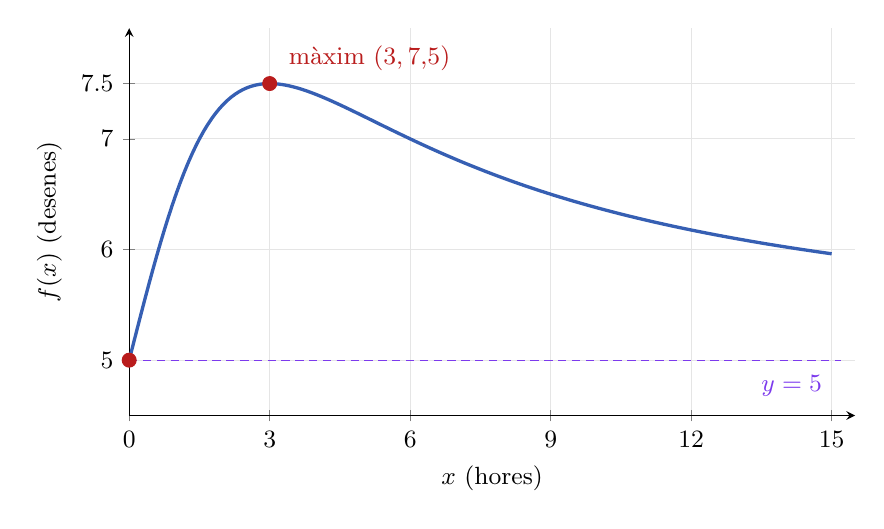
\begin{tikzpicture}
\begin{axis}[
  width=10.8cm,height=6.5cm,axis lines=left,
  xmin=0,xmax=15.5,ymin=4.5,ymax=8,
  xlabel={$x$ (hores)},ylabel={$f(x)$ (desenes)},
  xtick={0,3,6,9,12,15},ytick={5,6,7,7.5},
  grid=major,grid style={black!10},tick label style={font=\small},label style={font=\small},clip=false]
  \addplot[corba,very thick,domain=0:15,samples=180]{15*x/(9+x^2)+5};
  \addplot[asimptota,densely dashed,domain=0:15.2]{5};
  \addplot[only marks,mark=*,mark size=2.5pt,punt] coordinates {(0,5) (3,7.5)};
  \node[anchor=south west,font=\small,text=punt] at (axis cs:3.2,7.53) {màxim $(3,7{,}5)$};
  \node[anchor=north east,font=\small,text=asimptota] at (axis cs:15,4.95) {$y=5$};
\end{axis}
\end{tikzpicture}
\end{document}
